% !TeX root = Protokoll.tex
\subsection{Drehschieberpumpe}
In den Folgenden Abschnitten werden die, unter Verwendung der Drehschieberpumpe, aufgenommenen Messreihen 
zur Evakuierungskurve und der Leckratenmessung ausgewertet. Mit den Ergebnissen aus diesen, folgt im letzten Teil dieses 
Abschnitts die Betrachtung des Saugvermögens in Abhängigkeit des Druckes.

\subsubsection{Evakuierungskurve}

%Tabelle der Messwerte
\begin{table}[!h]
	\centering
	\begin{tabular}{cccccc}
		\toprule
		Druck & logarithm. Druck & gemittelte Zeit & Druck & logarithm. Druck & gemittelte Zeit\\
		$p$/\si{mbar} & $\frac{p-p_e}{p_0-p_e}$ & $\bar{t}$/\si{s} & $p$/\si{mbar} & $\frac{p-p_e}{p_0-p_e}$ & $\bar{t}$/\si{s}\\
\midrule
		\num{100(30)} & \num{0.0(0)} & \num{14(1)} & \num{1.0(3)} & \num{-4.6(4)} & \num{73(1)}\\
		\num{60(18)} & \num{-0.5(4)} & \num{25(1)} & \num{0.8(2)} & \num{-4.9(4)} & \num{75(1)}\\
		\num{40(12)} & \num{-0.9(4)} & \num{32(1)} & \num{0.6(2)} & \num{-5.1(4)} & \num{80(1)}\\
		\num{20(6)} & \num{-1.6(4)} & \num{41(1)} & \num{0.4(1)} & \num{-5.6(4)} & \num{88(1)}\\
		\num{10(3)} & \num{-2.3(4)} & \num{49(1)} & \num{0.20(6)} & \num{-6.3(4)} & \num{104(1)}\\
		\num{8(2)} & \num{-2.5(4)} & \num{51(1)} & \num{0.10(3)} & \num{-7.1(5)} & \num{121(1)}\\
		\num{6(2)} & \num{-2.8(4)} & \num{54(1)} & \num{0.08(2)} & \num{-7.4(5)} & \num{130(1)}\\
		\num{4(1)} & \num{-3.2(4)} & \num{58(1)} & \num{0.06(2)} & \num{-7.8(6)} & \num{149(1)}\\
		\num{2.0(6)} & \num{-3.9(4)} & \num{65(1)} & \num{0.04(1)} & \num{-8.5(7)} & \num{214(1)}\\
		\bottomrule
	\end{tabular}
	\caption{Werte der Messung der Evakuierungskurve unter Verwendung der Drehschieberpumpe.
                        Neben den gemessenen Drücken sind auch die logarithmierten Drücke und die gemittelten
                        Zeiten angegeben. Dabei sind die Fehler der Zeiten systematischen Ursprungs und wurden 
                        daher durch das Mitteln nicht reduziert. \label{tab:Evakuierungskurve_Drehschieber}}
\end{table}


%Exponential-Darstellung der Messdaten
{\begin{figure}[!h]
 \centering
 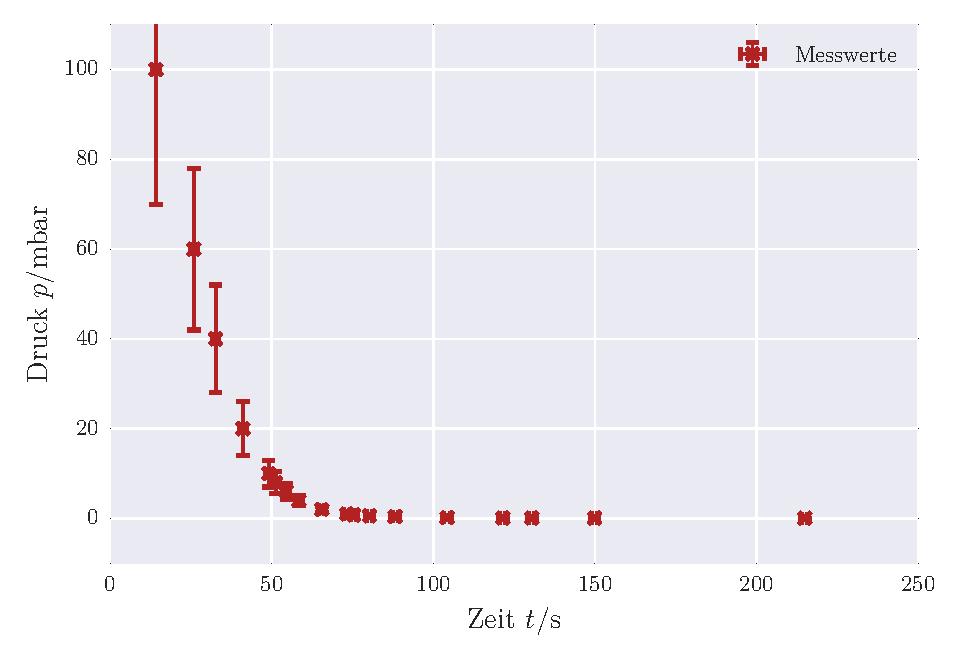
\includegraphics[scale=.9]{../Grafiken/Evakuierungskurve_Drehschieber_exp.pdf}
 \caption{Grafische Darstellung der aufgenommenen Evakuierungskurve der Drehschieberpumpe. \label{fig:evakuierungskurve_drehschieber_exp}}
 \end{figure} 
\FloatBarrier
%Logarithmische-Darstellung der Messdaten mit Fits
\begin{figure}[!h]
 \centering
 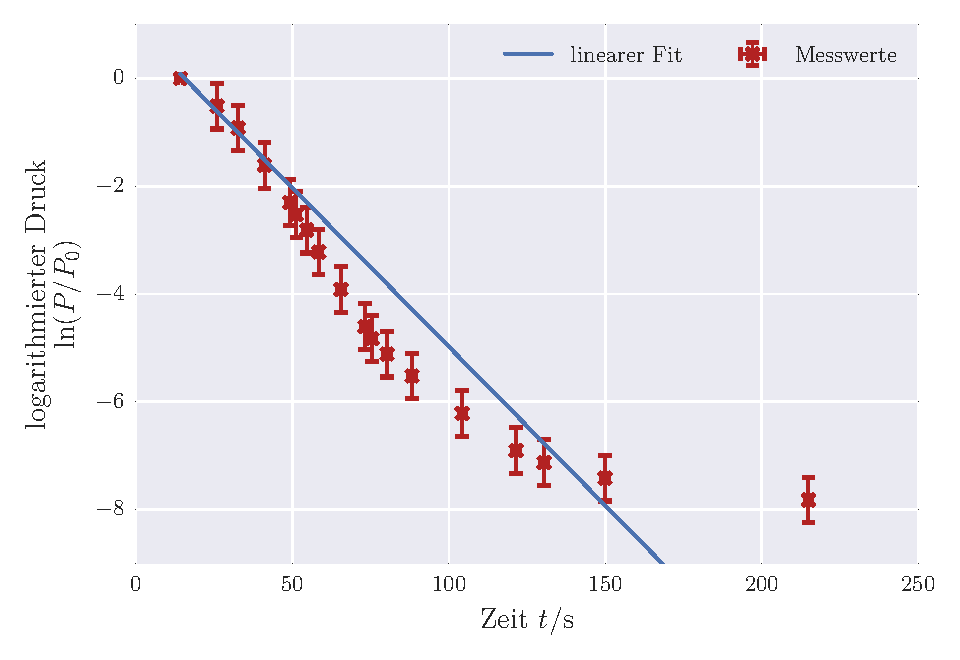
\includegraphics[scale=.80]{../Grafiken/Evakuierungskurve_Drehschieber_log_0.pdf}
 \caption{Grafische Darstellung der Evakuierungskurve mit logarithmierten Druckmesswerten und der Ausgleichsgrade für den ersten Druckbereich (\SI{100}{\milli\bar} bis \SI{20}{\milli\bar}) .\label{fig:evakuierungskurve_drehschieber_log_0}}
 \end{figure} 
\FloatBarrier
\begin{figure}[!h]
 \centering
 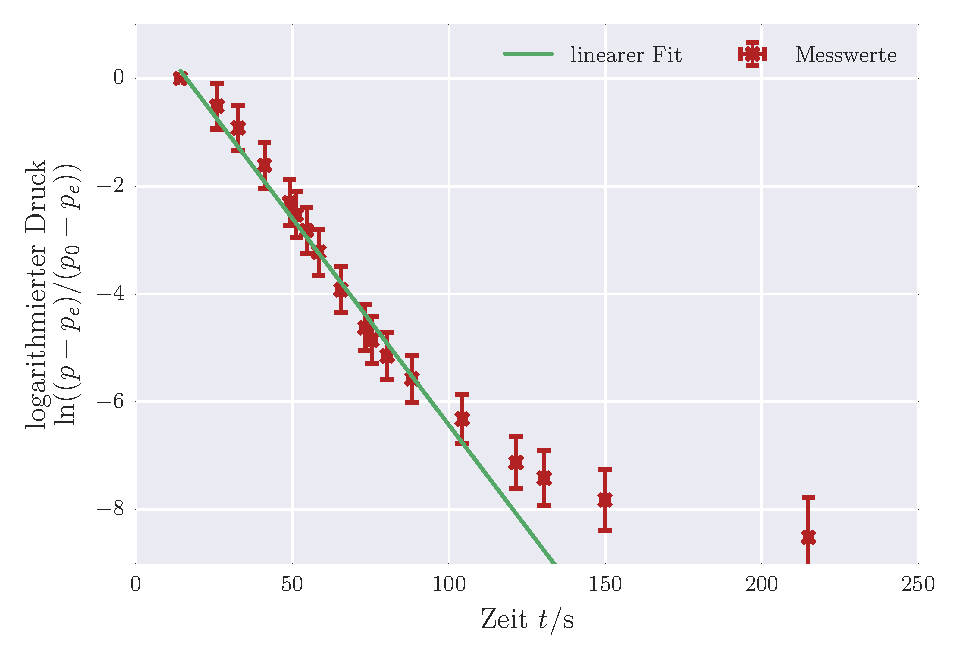
\includegraphics[scale=.80]{../Grafiken/Evakuierungskurve_Drehschieber_log_1.pdf}
 \caption{Grafische Darstellung der Evakuierungskurve mit logarithmierten Druckmesswerten und der Ausgleichsgrade für den zweiten Druckbereich (\SI{10}{\milli\bar} bis \SI{0.2}{\milli\bar}) \label{fig:evakuierungskurve_drehschieber_log_1}}
 \end{figure} 
\FloatBarrier
\begin{figure}[!h]
 \centering
 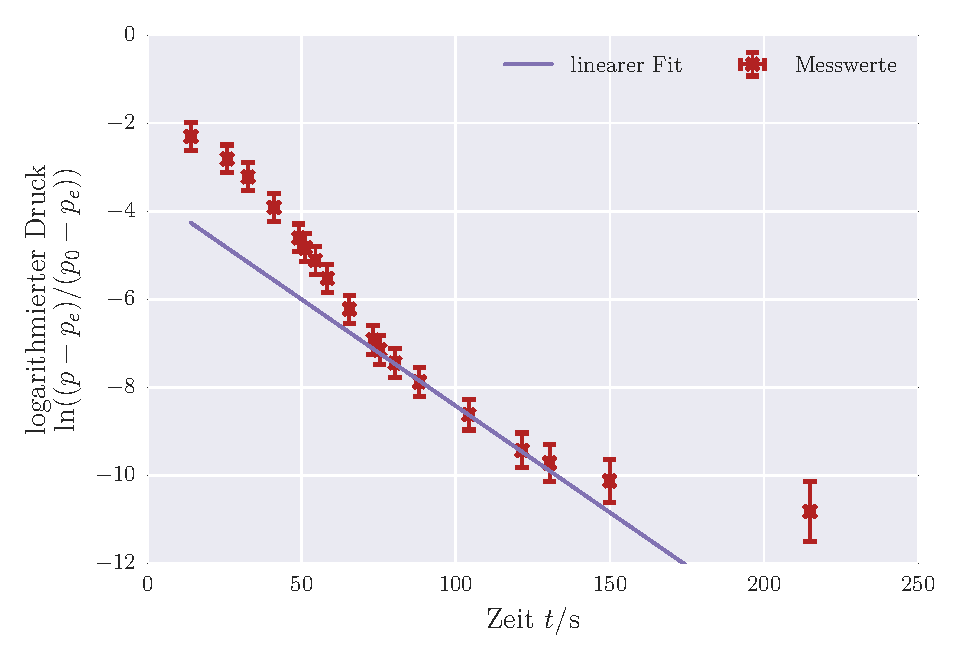
\includegraphics[scale=.80]{../Grafiken/Evakuierungskurve_Drehschieber_log_2.pdf}
 \caption{Grafische Darstellung der Evakuierungskurve mit logarithmierten Druckmesswerten und der Ausgleichsgrade für den dritten Druckbereich (\SI{0.1}{\milli\bar} bis \SI{0.04}{\milli\bar}) \label{fig:evakuierungskurve_drehschieber_log_2}}
 \end{figure} 
\FloatBarrier}

\subsubsection{Leckratenmessung}

%Tabelle zur Leckratenmessung
\begin{table}[!h]
	\centering
	\subfloat{
	\begin{tabular}{cccc}
		\toprule
		\multicolumn{2}{c}{1.Messreihe $P_g = \SI{0.10(3)}{\milli\bar}$} & \multicolumn{2}{c}{2.Messreihe $P_g = \SI{0.20(6)}{\milli\bar}$} \\\cmidrule(rl){1-2}\cmidrule(rl){3-4}
		Druck & gemittelte Zeit & Druck & gemittelte Zeit\\
		$p$/\si{mbar} & $\bar{t}$/\si{s} & $p$/\si{mbar} & $\bar{t}$/\si{s}\\
\midrule
		\num{0.20(6)} & \num{12(1)} & \num{0.4(1)} & \num{17(1)}\\
		\num{0.4(1)} & \num{64(1)} & \num{0.6(2)} & \num{46(1)}\\
		\num{0.6(2)} & \num{128(1)} & \num{0.8(2)} & \num{72(1)}\\
		\bottomrule
%	\end{tabular}
%	}\\
%	\subfloat{
%	\begin{tabular}{cccc}
		\toprule
		\multicolumn{2}{c}{3.Messreihe $P_g = \SI{0.4(1)}{\milli\bar}$ } & \multicolumn{2}{c}{4.Messreihe $P_g = \SI{0.8(2)}{\milli\bar}$} \\\cmidrule(rl){1-2}\cmidrule(rl){3-4}
		Druck & gemittelte Zeit & Druck & gemittelte Zeit\\
		$p$/\si{mbar} & $\bar{t}$/\si{s} & $p$/\si{mbar} & $\bar{t}$/\si{s}\\
		\midrule
		\num{0.6(2)} & \num{9(1)} & \num{2.0(6)} & \num{12(1)}\\
		\num{0.8(2)} & \num{18(1)} & \num{4(1)} & \num{34(1)}\\
		\num{1.0(3)} & \num{42(1)} & \num{6(2)} & \num{55(1)}\\
		\bottomrule
	\end{tabular}
	}
	
	\caption{Werte der Leckratenmessung unter Verwendung der Drehschieberpumpe.
                        Neben den gemessenen Drücken sind die gemittelten Zeiten angegeben. 
                        Dabei sind die Fehler der Zeiten systematischen Ursprungs und wurden 
                        daher durch das Mitteln nicht reduziert. \label{tab:Leckratenmessung_Drehschieber_0}}
\end{table}


%Grafiken der Leckratenmessung
\begin{figure}[!h]
 \centering
 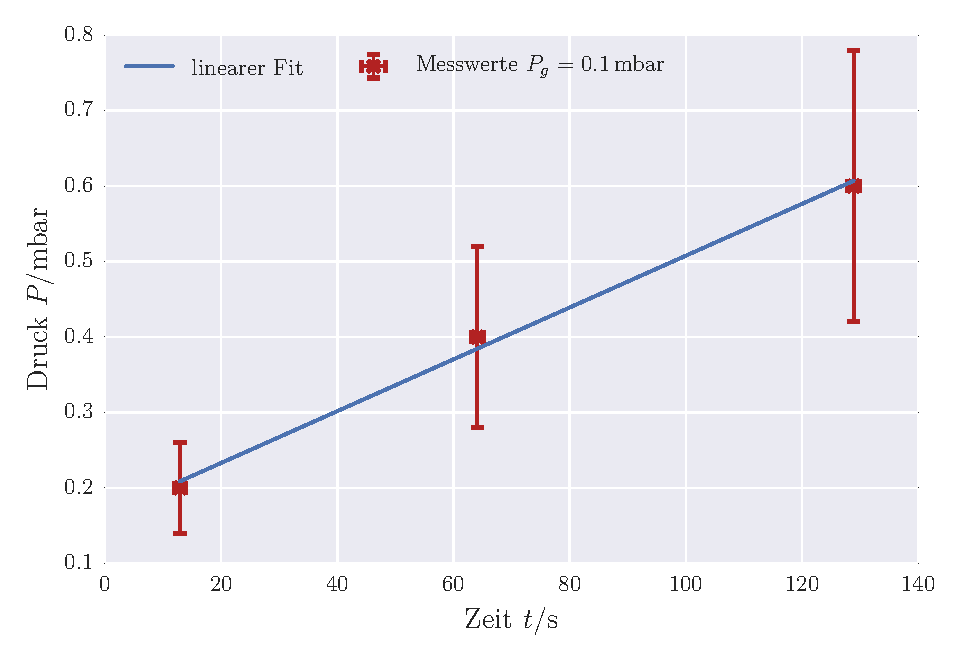
\includegraphics[scale=0.8]{../Grafiken/Leckrate_Drehschieber_0.pdf}
 \caption{Graphische Darstellung der Druckmesswerte in Abhängigkeit von der Zeit, aus der 1. Messreihe, und der
 	entsprechenden Ausgleichsgeraden. Der für die Messreihe eingestellte Gleichgewichtsdruck ist angegeben.\label{fig:leckrate_drehschieber_0}}
 \end{figure} 
\FloatBarrier
%Logarithmische-Darstellung der Messdaten mit Fits
\begin{figure}[!h]
 \centering
 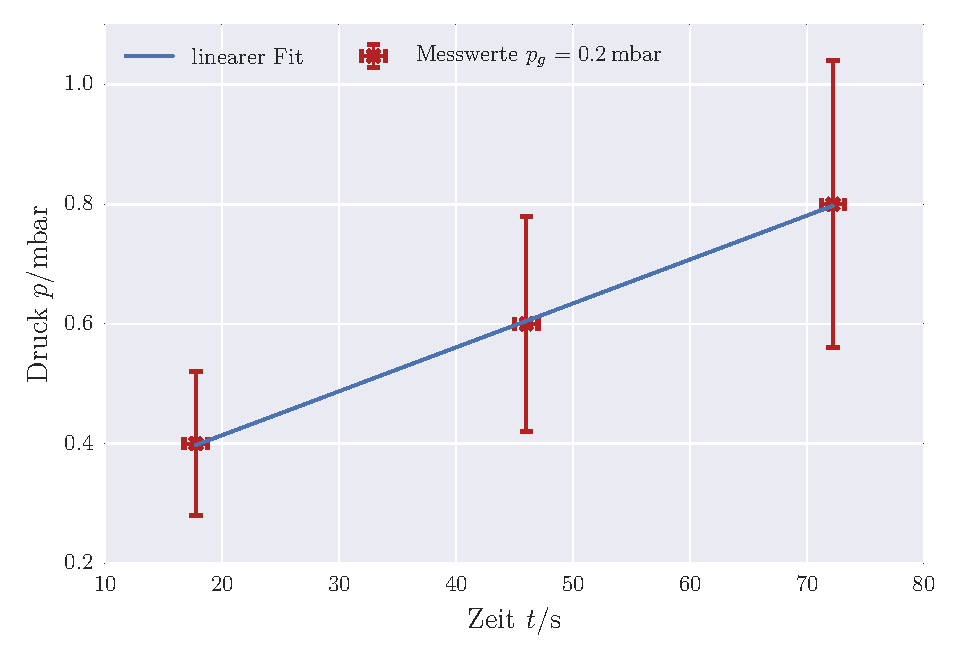
\includegraphics[scale=0.9]{../Grafiken/Leckrate_Drehschieber_1.pdf}
 \caption{Graphische Darstellung der Druckmesswerte in Abhängigkeit von der Zeit, aus der 2. Messreihe, und der
 	entsprechenden Ausgleichsgeraden. Der für die Messreihe eingestellte Gleichgewichtsdruck ist angegeben.\label{fig:leckrate_drehschieber_1}}
 \end{figure} 
\FloatBarrier
\begin{figure}[!h]
 \centering
 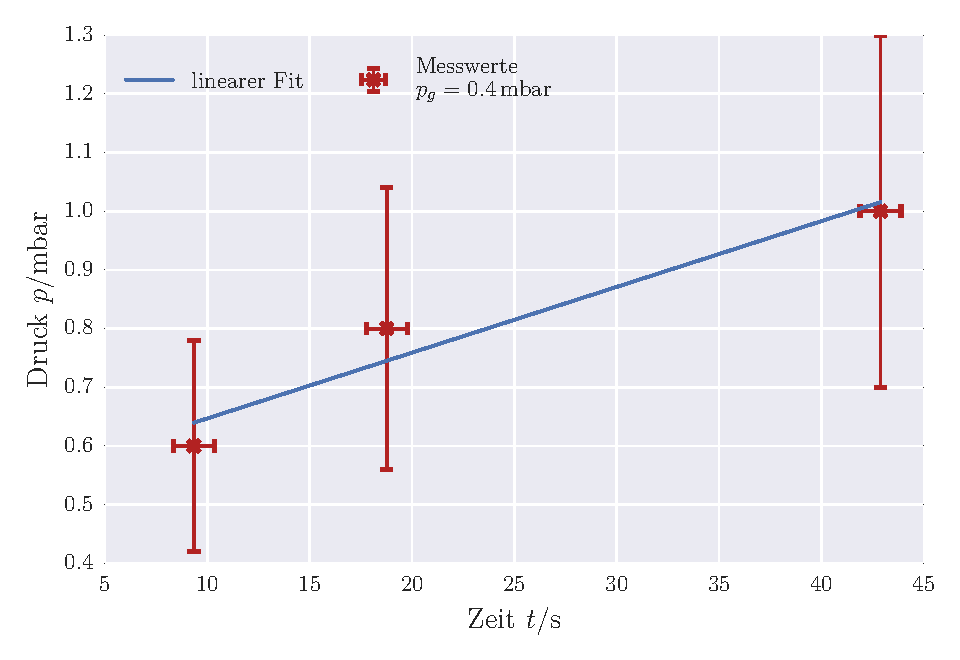
\includegraphics[scale=0.8]{../Grafiken/Leckrate_Drehschieber_2.pdf}
 \caption{Graphische Darstellung der Druckmesswerte in Abhängigkeit von der Zeit, aus der 3. Messreihe, und der
 	entsprechenden Ausgleichsgeraden. Der für die Messreihe eingestellte Gleichgewichtsdruck ist angegeben und als Messwert für $t=0$ mit eingetragen. Dieser ist grau dargestellt, da er für die 
 	Berechnung der Ausgleichsgeraden nicht verwendet wurde. \label{fig:leckrate_drehschieber_2}}
 \end{figure} 
\FloatBarrier
\begin{figure}[!h]
 \centering
 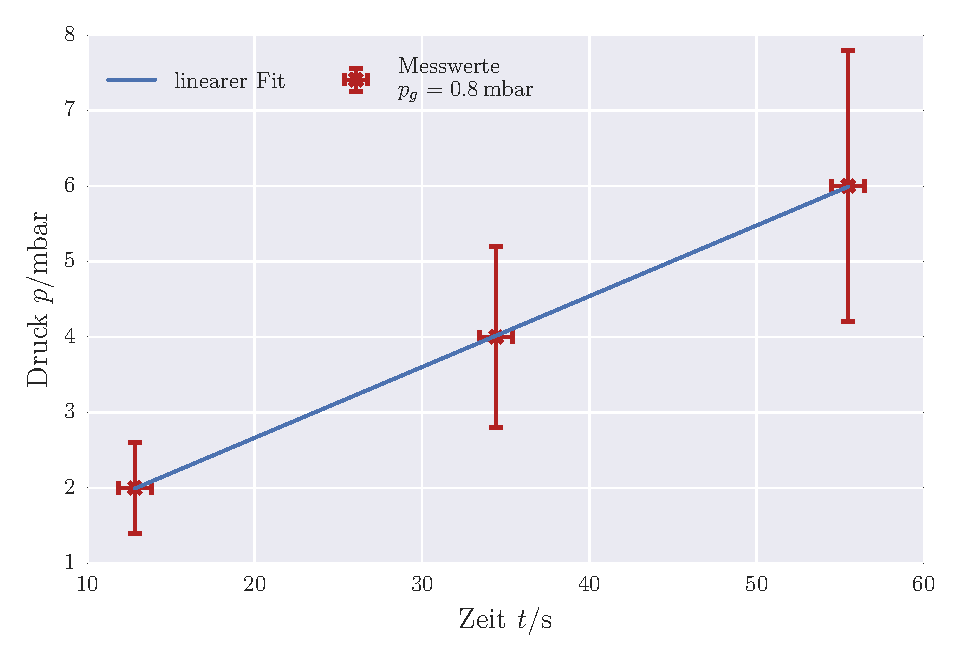
\includegraphics[scale=0.8]{../Grafiken/Leckrate_Drehschieber_3.pdf}
 \caption{Graphische Darstellung der Druckmesswerte in Abhängigkeit von der Zeit, aus der 4. Messreihe, und der
 entsprechenden Ausgleichsgeraden. Der für die Messreihe eingestellte Gleichgewichtsdruck ist angegeben und als Messwert für $t=0$ mit eingetragen. Dieser ist grau dargestellt, da er für die 
 Berechnung der Ausgleichsgeraden nicht verwendet wurde. \label{fig:leckrate_drehschieber_3}}
 \end{figure} 
\FloatBarrier
\subsubsection{Saugvermögen}
%Tabelle zum Saugvermögen
\begin{table}[!h]
	\centering
	\begin{tabular}{cccc}
		\toprule
		Druck & Saugvermögen & Druck & Saugvermögen\\
		$p$/\si{mbar} & $S$/\si{ls^{-1}} & $p$/\si{mbar} & $S$/\si{ls^{-1}}\\
\midrule
		\num{0.08(2)} & \num{0.14(2)} & \num{0.6(2)} & \num{0.49(4)}\\
		\num{0.10(3)} & \num{0.3(1)} & \num{0.8(2)} & \num{1.2(4)}\\
		\num{0.20(6)} & \num{0.4(1)} & \num{4(1)} & \num{0.97(6)}\\
		\num{0.4(1)} & \num{0.3(1)} & \num{60(18)} & \num{0.50(5)}\\
		\bottomrule
	\end{tabular}
	\caption{Aus den vorherigen Messergebnissen berechnet Werte für das 
                        Saugvermögen der Drehschieberpumpe in Abhängigkeit des jeweiligen Druckes. \label{tab:Saugvermoegen_Drehschieber}}
\end{table}


%Grafik des Saugvermögens
\begin{figure}[!h]
 \centering
 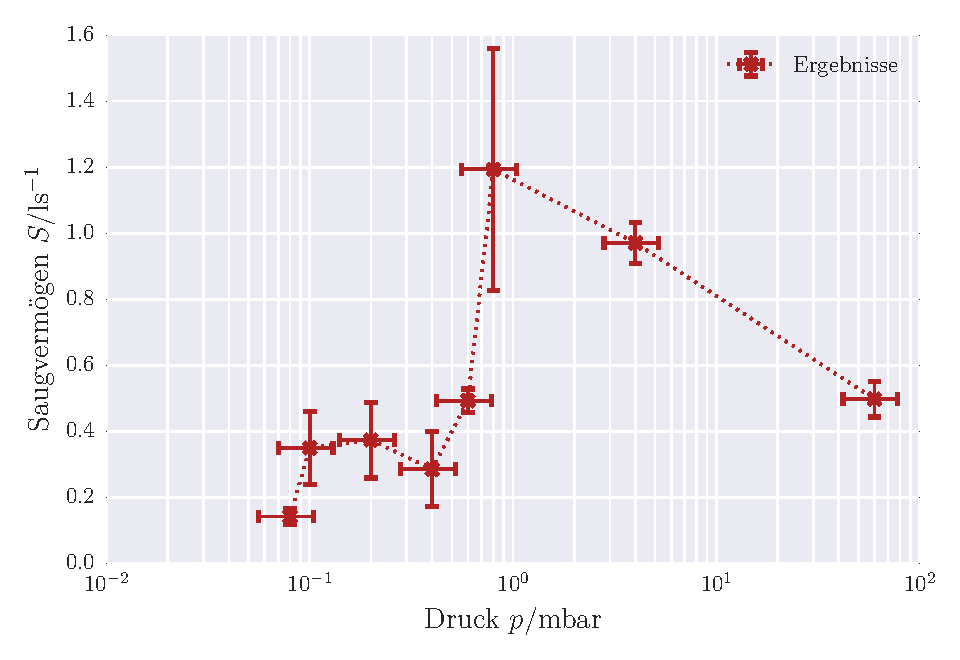
\includegraphics[scale=0.8]{../Grafiken/Saugvermoegen_Drehschieber.pdf}
 \caption{Grafische Darstellung der Ergebnisse für das Saugvermögen aus den vorangegangenen Messreihen in 
 Abhängigkeit des Druckes bei dem sich dieses Saugvermögen ergab. \label{fig:saugvermögen_drehschieber}}
 \end{figure} 
\FloatBarrier

\subsection{Turbopumpe}
In den Folgenden Abschnitten werden die, unter Verwendung der Turbopumpe, aufgenommenen Messreihen 
zur Evakuierungskurve und der Leckratenmessung ausgewertet. Mit den Ergebnissen aus diesen, folgt im letzten Teil dieses 
Abschnitts die Betrachtung des Saugvermögens in Abhängigkeit des Druckes.

\subsubsection{Evakuierungskurve}

%Tabelle der Messwerte
\begin{table}[!h]
	\centering
	\begin{tabular}{cccccc}
		\toprule
		Druck & logarithm. Druck & gemittelte Zeit & Druck & logarithm. Druck & gemittelte Zeit\\
		$p$/\si{10^{-8}\,bar} & $\frac{p-p_e}{p_0-p_e}$ & $\bar{t}$/\si{s} & $p$/\si{10^{-8}\,bar} & $\frac{p-p_e}{p_0-p_e}$ & $\bar{t}$/\si{s}\\
\midrule
		\num{80(8)} & \num{0.0(0)} & \num{5(1)} & \num{9.0(9)} & \num{-2.4(2)} & \num{18(1)}\\
		\num{70(7)} & \num{-0.1(1)} & \num{6(1)} & \num{8.0(8)} & \num{-2.5(2)} & \num{20(1)}\\
		\num{59(6)} & \num{-0.3(1)} & \num{6(1)} & \num{7.0(7)} & \num{-2.7(2)} & \num{22(1)}\\
		\num{50(5)} & \num{-0.5(1)} & \num{7(1)} & \num{6.0(6)} & \num{-2.9(2)} & \num{24(1)}\\
		\num{40(4)} & \num{-0.7(1)} & \num{8(1)} & \num{5.0(5)} & \num{-3.1(2)} & \num{28(1)}\\
		\num{29(3)} & \num{-1.0(1)} & \num{9(1)} & \num{4.0(4)} & \num{-3.5(2)} & \num{34(1)}\\
		\num{20(2)} & \num{-1.4(1)} & \num{12(1)} & \num{3.0(3)} & \num{-4.0(3)} & \num{48(1)}\\
		\num{10(1)} & \num{-2.2(2)} & \num{17(1)}\\
		\bottomrule
	\end{tabular}
	\caption{Werte der Messung der Evakuierungskurve unter Verwendung der Turbopumpe.
                        Neben den gemessenen Drücken sind auch die logarithmierten Drücke und die gemittelten
                        Zeiten angegeben. Dabei sind die Fehler der Zeiten systematischen Ursprungs und wurden 
                        daher durch das Mitteln nicht reduziert. \label{tab:Evakuierungskurve_Turbo}}
\end{table}


%Exponential-Darstellung der Messdaten
\begin{figure}[!h]
 \centering
 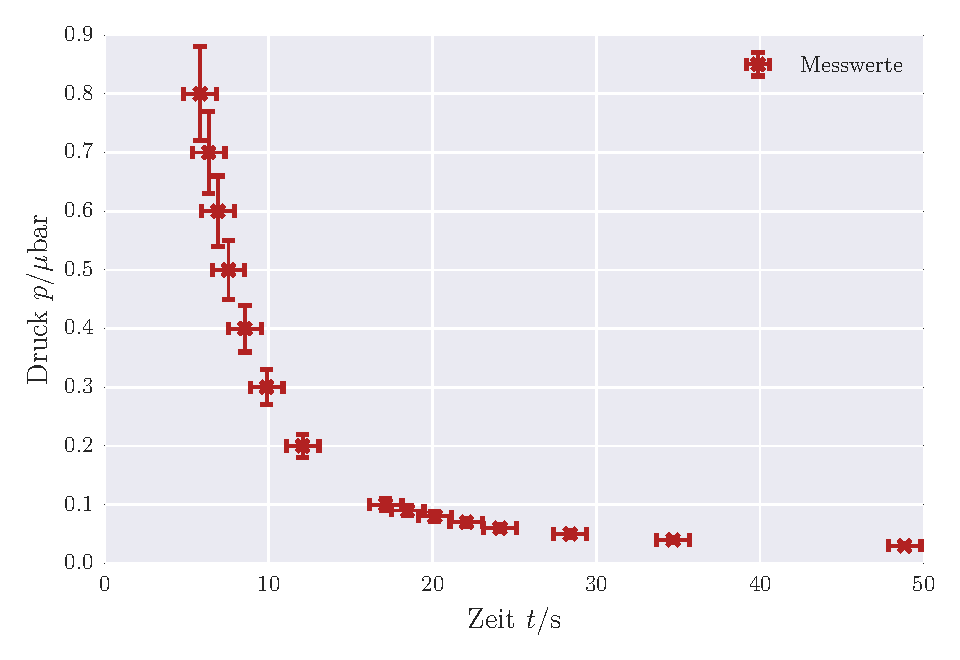
\includegraphics[scale=0.9]{../Grafiken/Evakuierungskurve_Turbo_exp.pdf}
 \caption{Grafische Darstellung der aufgenommenen Evakuierungskurve der Turbopumpe.\label{fig:evakuierungskurve_turbo_exp}}
 \end{figure} 
\FloatBarrier
%Logarithmische-Darstellung der Messdaten mit Fits
\begin{figure}[!h]
 \centering
 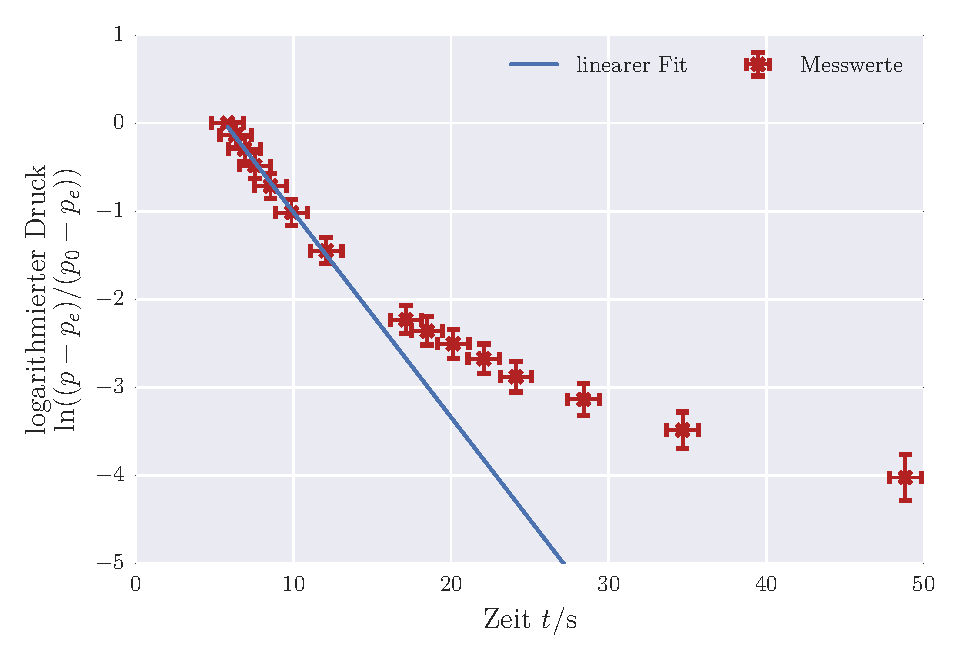
\includegraphics[scale=0.8]{../Grafiken/Evakuierungskurve_Turbo_log_0.pdf}
 \caption{Grafische Darstellung der Evakuierungskurve mit logarithmierten Druckmesswerten und der Ausgleichsgrade für den ersten Druckbereich (\SI{0.8}{\micro\bar} bis \SI{0.6}{\micro\bar})\label{fig:evakuierungskurve_turbo_log_0}}
 \end{figure} 
\FloatBarrier
\begin{figure}[!h]
 \centering
 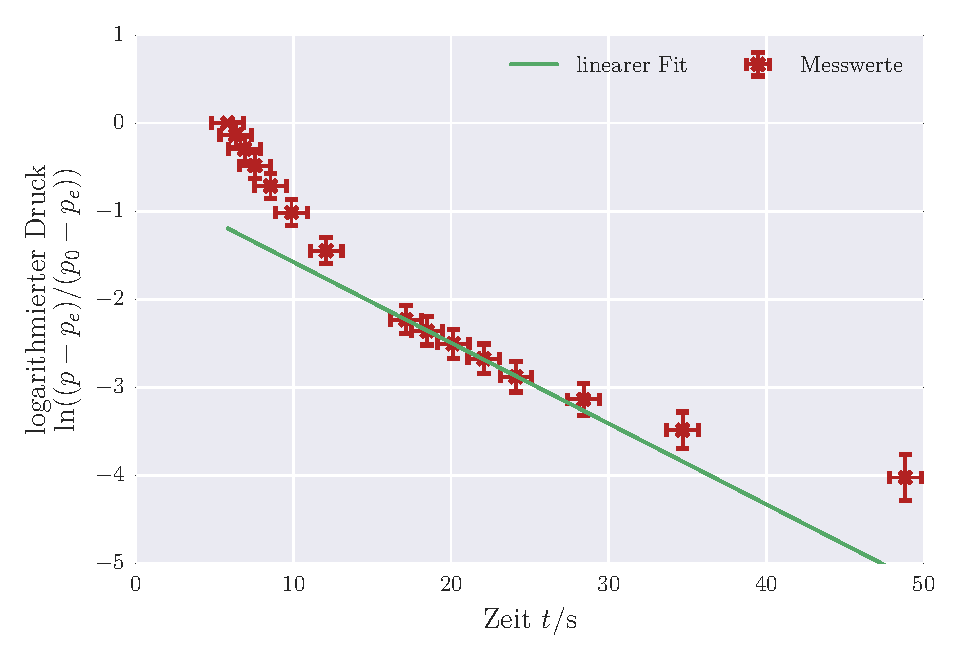
\includegraphics[scale=0.8]{../Grafiken/Evakuierungskurve_Turbo_log_1.pdf}
 \caption{Grafische Darstellung der Evakuierungskurve mit logarithmierten Druckmesswerten und der Ausgleichsgrade für den zweiten Druckbereich (\SI{0.5}{\micro\bar} bis \SI{0.2}{\micro\bar})\label{fig:evakuierungskurve_turbo_log_1}}
 \end{figure} 
\FloatBarrier
\begin{figure}[!h]
 \centering
 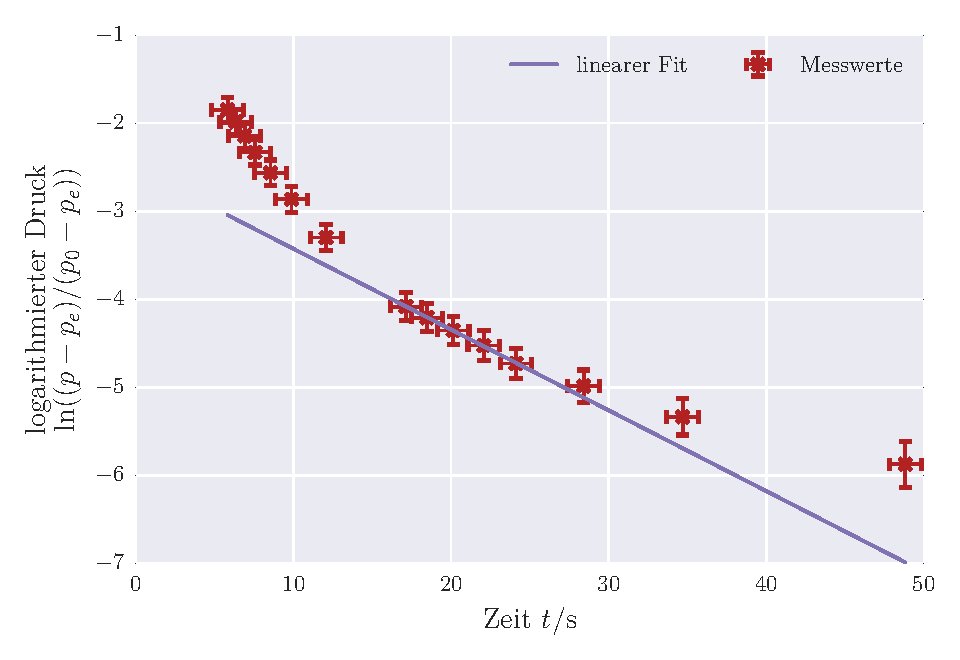
\includegraphics[scale=0.9]{../Grafiken/Evakuierungskurve_Turbo_log_2.pdf}
 \caption{Grafische Darstellung der Evakuierungskurve mit logarithmierten Druckmesswerten und der Ausgleichsgrade für den dritten Druckbereich (\SI{50}{\nano\bar} bis \SI{30}{\nano\bar})\label{fig:evakuierungskurve_turbo_log_2}}
 \end{figure} 
\FloatBarrier

\subsubsection{Leckratenmessung}
% Tabelle der Lecktratenmessung
\begin{table}[!h]
	\centering
	\subfloat{
	\begin{tabular}{cccc}
		\toprule
		\multicolumn{2}{c}{1.Messreihe $P_g = \SI{4.0(4)e-08}{\bar}$} & \multicolumn{2}{c}{2.Messreihe $P_g = \SI{6.0(6)e-08}{\bar}$} \\\cmidrule(rl){1-2}\cmidrule(rl){3-4}
		Druck & gemittelte Zeit & Druck & gemittelte Zeit\\
		$p$/\si{10^{-8}bar} & $\bar{t}$/\si{s} & $p$/\si{10^{-8}bar} & $\bar{t}$/\si{s}\\
		\midrule
		\num{20(2)} & \num{5(1)} & \num{20(2)} & \num{1(1)}\\
		\num{30(3)} & \num{8(1)} & \num{30(3)} & \num{2(1)}\\
		\num{40(4)} & \num{11(1)} & \num{40(4)} & \num{4(1)}\\
					&			& \num{50(5)} & \num{6(1)}\\
		\bottomrule
%	\end{tabular}
%	}\\
%	\subfloat{
%	\begin{tabular}{cccc}
		\toprule
		\multicolumn{2}{c}{3.Messreihe $P_g = \SI{8.0(8)e-08}{\bar}$} & \multicolumn{2}{c}{4.Messreihe $P_g = \SI{1.0(1)e-07}{\bar}$} \\\cmidrule(rl){1-2}\cmidrule(rl){3-4}
		Druck & gemittelte Zeit & Druck & gemittelte Zeit\\
		$p$/\si{10^{-8}bar} & $\bar{t}$/\si{s} & $p$/\si{10^{-8}bar} & $\bar{t}$/\si{s}\\
		\midrule
		\num{30(9)} & \num{1(1)} & \num{40(12)} & \num{2(1)}\\
		\num{40(12)} & \num{2(1)} & \num{50(15)} & \num{2(1)}\\
		\num{50(15)} & \num{3(1)} & \num{60(18)} & \num{3(1)}\\
		\num{60(18)} & \num{6(1)} & \num{70(21)} & \num{4(1)}\\
		\bottomrule
	\end{tabular}
	}
	
	\caption{Werte der Leckratenmessung unter Verwendung der Turbopumpe.
		Neben den gemessenen Drücken sind die gemittelten Zeiten angegeben. 
		Dabei sind die Fehler der Zeiten systematischen Ursprungs und wurden 
		daher durch das Mitteln nicht reduziert. \label{tab:Leckratenmessung_Turbo}}
\end{table}


%Grafiken der Leckratenmessung
\begin{figure}[!h]
 \centering 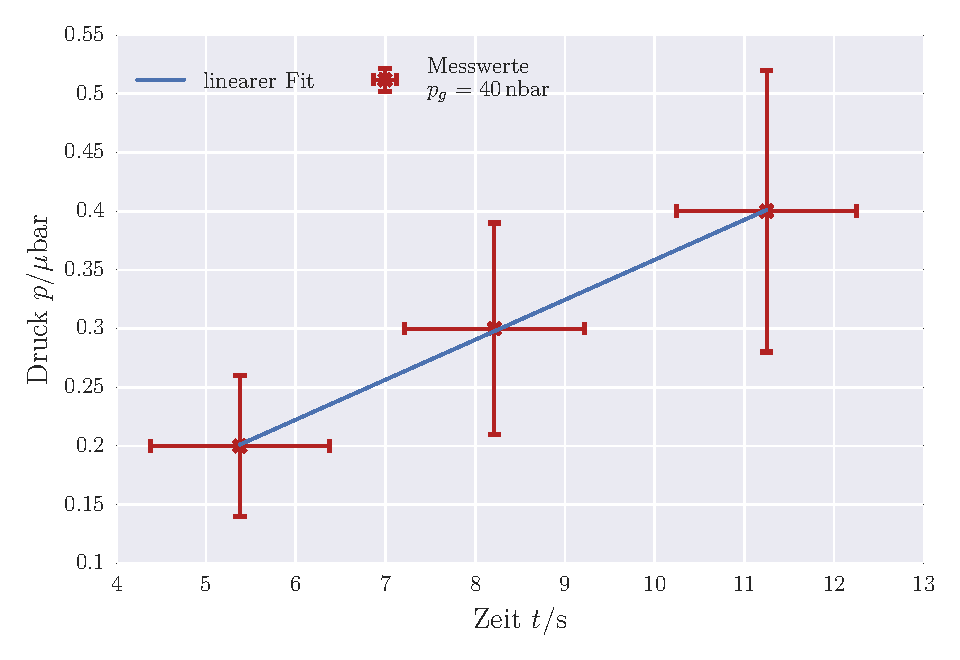
\includegraphics[scale=0.8]{../Grafiken/Leckrate_Turbo_0.pdf}                                                          
 \caption{Graphische Darstellung der Druckmesswerte in Abhängigkeit von der Zeit, aus der 1. Messreihe, und der
 	entsprechenden Ausgleichsgeraden. Der für die Messreihe eingestellte Gleichgewichtsdruck ist angegeben. \label{fig:leckrate_turbo_0}}
 \end{figure} 
\FloatBarrier

\begin{figure}[!h]
 \centering
 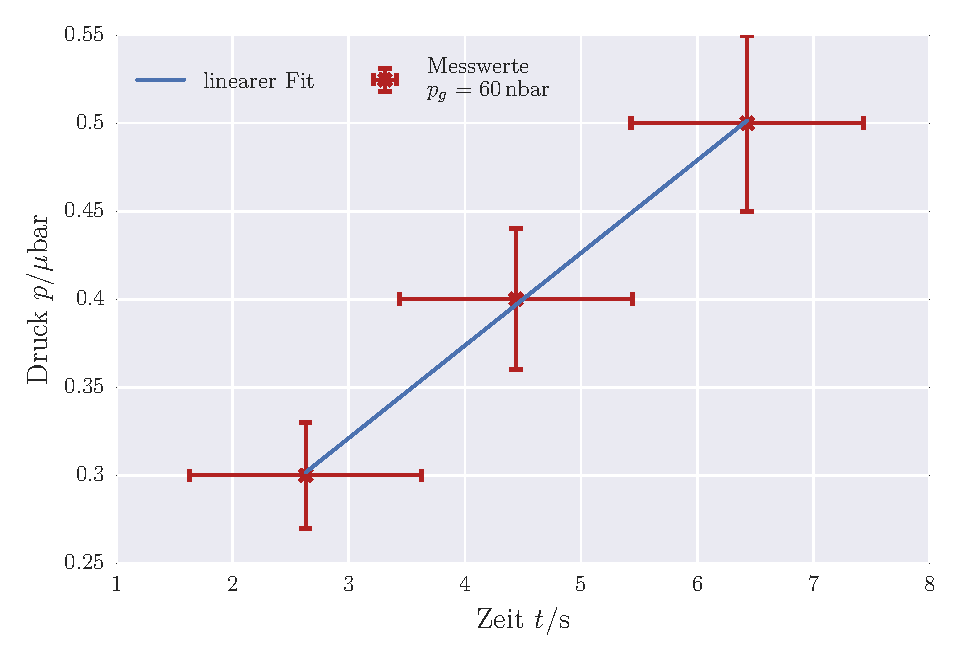
\includegraphics[scale=0.65]{../Grafiken/Leckrate_Turbo_1.pdf}	
 \caption{Graphische Darstellung der Druckmesswerte in Abhängigkeit von der Zeit, aus der 2. Messreihe, und der
 	entsprechenden Ausgleichsgeraden. Der für die Messreihe eingestellte Gleichgewichtsdruck ist angegeben und als Messwert für $t=0$ mit eingetragen. Dieser ist grau dargestellt, da er für die 
 	Berechnung der Ausgleichsgeraden nicht verwendet wurde. Diese Auslassung wurde vorgenommen, da
 	der tatsächliche Druck bei $t=0$, durch den plötzlichen Druckanstieg bei Schließung des Ventils zur Pumpe, von dem
 	gemessenen Druck bei offenem Ventil abweicht.
 \label{fig:leckrate_turbo_1}}
 \end{figure} 
\FloatBarrier
\begin{figure}[!h]
 \centering
 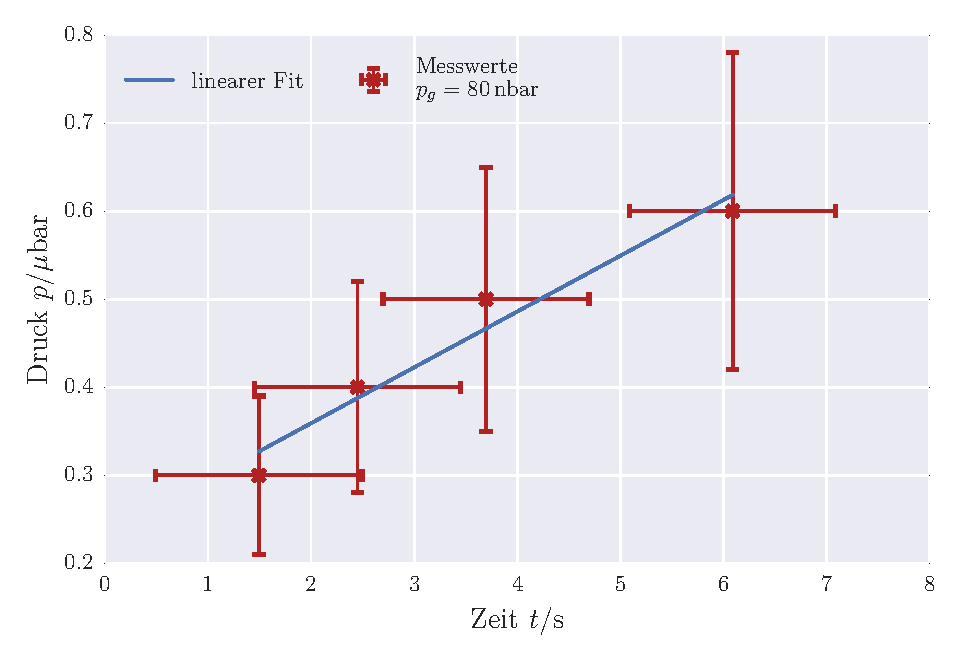
\includegraphics[scale=0.65]{../Grafiken/Leckrate_Turbo_2.pdf}
 \caption{Graphische Darstellung der Druckmesswerte in Abhängigkeit von der Zeit, aus der 3. Messreihe, und der
 	entsprechenden Ausgleichsgeraden. Der für die Messreihe eingestellte Gleichgewichtsdruck ist angegeben und als Messwert für $t=0$ mit eingetragen. Dieser ist grau dargestellt, da er für die 
 	Berechnung der Ausgleichsgeraden nicht verwendet wurde. Diese Auslassung wurde vorgenommen, da
 	der tatsächliche Druck bei $t=0$, durch den plötzlichen Druckanstieg bei Schließung des Ventils zur Pumpe, von dem
 	gemessenen Druck bei offenem Ventil abweicht.  \label{fig:leckrate_turbo_2}}
 \end{figure} 
\FloatBarrier
\begin{figure}[!h]
 \centering
 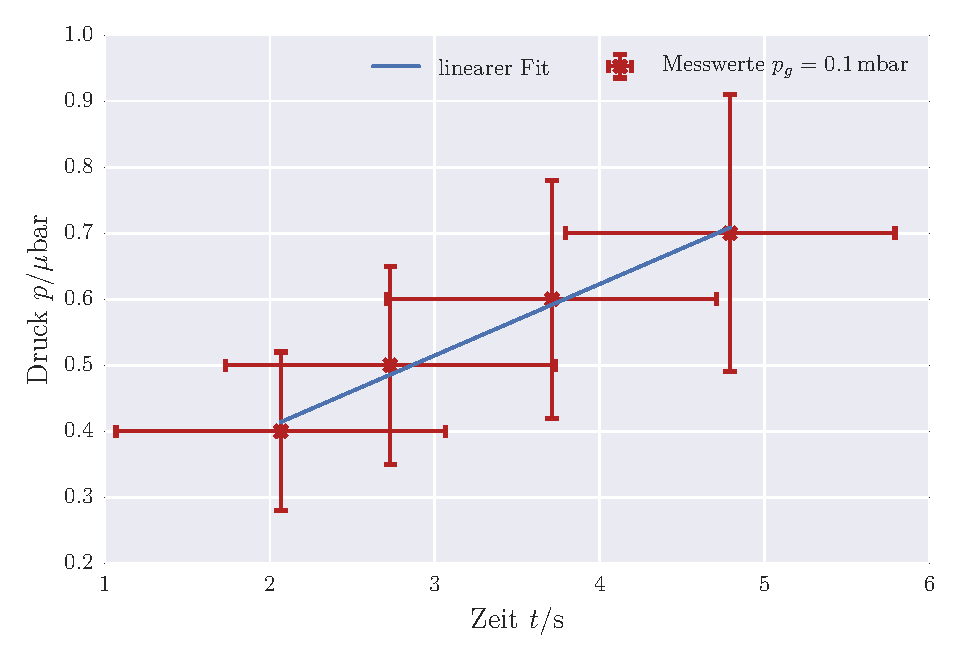
\includegraphics[scale=0.65]{../Grafiken/Leckrate_Turbo_3.pdf}
 \caption{Graphische Darstellung der Druckmesswerte in Abhängigkeit von der Zeit, aus der 4. Messreihe, und der
 	entsprechenden Ausgleichsgeraden. Der für die Messreihe eingestellte Gleichgewichtsdruck ist angegeben und als Messwert für $t=0$ mit eingetragen. Dieser ist grau dargestellt, da er für die 
 	Berechnung der Ausgleichsgeraden nicht verwendet wurde. Diese Auslassung wurde vorgenommen, da
 	der tatsächliche Druck bei $t=0$, durch den plötzlichen Druckanstieg bei Schließung des Ventils zur Pumpe, von dem
 	gemessenen Druck bei offenem Ventil abweicht.  \label{fig:leckrate_turbo_3}}
 \end{figure} 
\FloatBarrier

\subsubsection{Saugvermögen}
%Tabelle zum Saugvermögen
\begin{table}[!h]
	\centering
	\begin{tabular}{cccc}
		\toprule
		Druck & Saugvermögen & Druck & Saugvermögen\\
		$p$/\si{10^{-8}\,bar} & $S$/\si{ls^{-1}} & $p$/\si{10^{-8}\,bar} & $S$/\si{ls^{-1}}\\
\midrule
		\num{4.0(4)} & \num{8(1)} & \num{9.0(9)} & \num{0.92(6)}\\
		\num{5.0(5)} & \num{0.43(5)} & \num{10(1)} & \num{10(2)}\\
		\num{6.0(6)} & \num{8(1)} & \num{40(4)} & \num{2.1(2)}\\
		\num{8.0(8)} & \num{8(2)} & \num{70(7)} & \num{2.7(2)}\\
		\bottomrule
	\end{tabular}
	\caption{Aus den vorherigen Messergebnissen berechnet Werte für das 
                       Saugvermögen der Turbopumpe in Abhängigkeit des jeweiligen Druckes. \label{tab:Saugvermoegen_Drehschieber}}
\end{table}


%Grafik des Saugvermögens
\begin{figure}[!h]
 \centering
 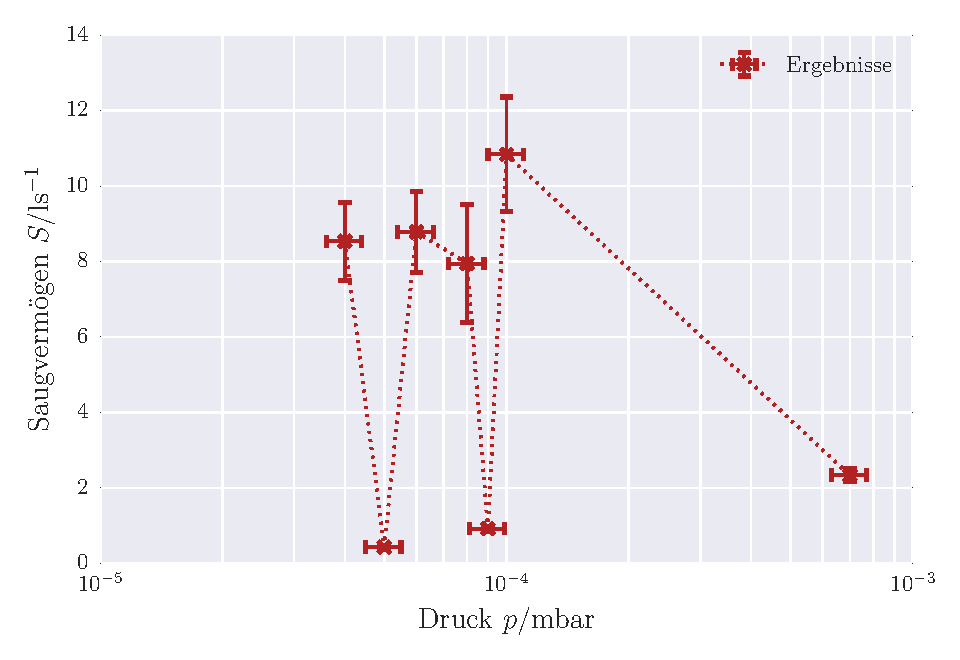
\includegraphics[scale=0.9]{../Grafiken/Saugvermoegen_Turbo.pdf}
 \caption{Grafische Darstellung der Ergebnisse für das Saugvermögen aus den vorangegangenen Messreihen in 
 	Abhängigkeit des Druckes bei dem sich dieses Saugvermögen ergab. \label{fig:saugvermögen_turbo}}
 \end{figure} 
\FloatBarrier









